
\section{Algoritmi}
\label{cap:algorithms}

\subsection{TSP 2-approssimato basato sul Minimum Spanning Tree}

La versione vista a lezione di questo algoritmo prevede i seguenti step:

\begin{enumerate}
    \item Selezionare un vertice radice $root$ arbitrario;
    \item Ricavare l'MST del grafo in input a partire da $root$, utilizzando ad esempio l'algoritmo di Prim;
    \item Eseguire una visita pre-order dell'MST ricavato al passo precedente;
    \item Aggiungere la radice $root$ pre-order alla fine della lista ritornata dalla visita pre-order.
    \item Calcolare il peso totale del circuito ricavato nei 2 passi precedenti e restituire il risultato.
\end{enumerate}

\noindent Il listato \ref{listing:tsp2approx} contiene la nostra implementazione dell'algoritmo, step per step.\\

\begin{listing}[!ht]
\begin{minted}{c++}
    // Step 1
    random_generator::IntegerRandomGenerator random(0, distance_matrix.size() - 1);
    const size_t root = random();

    // Step 2
    std::vector<Edge> mst(mst::prim_binary_heap_mst(distance_matrix, root));

    // Step 3, 4
    DFS dfs(std::move(mst));
    const auto circuit = dfs.preorder_traversal_rec();
    
    // Funzione lambda che calcola la distanza tra due vertici
    const auto get_distance = [&distance_matrix](const size_t x, const size_t y) {
        return distance_matrix.at(x, y);
    };
    
    // Step 5
    return utils::sum_weights_in_circuit(circuit.cbegin(), circuit.cend(), get_distance);
\end{minted}
\caption{Implementazione di TSP 2-approssimato. I commenti del file originale sono stati omessi per una maggiore compattezza.}
\label{listing:tsp2approx}
\end{listing}

\noindent L'algoritmo TSP 2-approssimato è stato implementato a partire dallo pseudo codice visto in classe. \\

\subsubsection{Osservazioni}

\begin{itemize}
    \item Abbiamo usato l'algoritmo di Prim perché è più adatto rispetto a Kruskal quando il grafo è rappresentato come matrice di adiacenza. Kruskal infatti richiede di estrarre la lista di lati ordinata in modo ascendente rispetto al peso all'inizio dell'algoritmo, mentre Prim richiede di estrarre solo la lista dei vertici. Ricordiamo che in un grafo completo vale l'equivalenza \complexityCompleteGraph{}.
    
    \item La coda di priorità usata dall'algoritmo di Prim è stata implementata con una Min Heap binaria.
\end{itemize}

\subsection{Held e Karp}

Riportiamo lo pseudocodice dell'algortimo di Held e Karp in Figura \ref{fig:heldkarp-pseudocode}.

\begin{figure}[h]
	\centering
	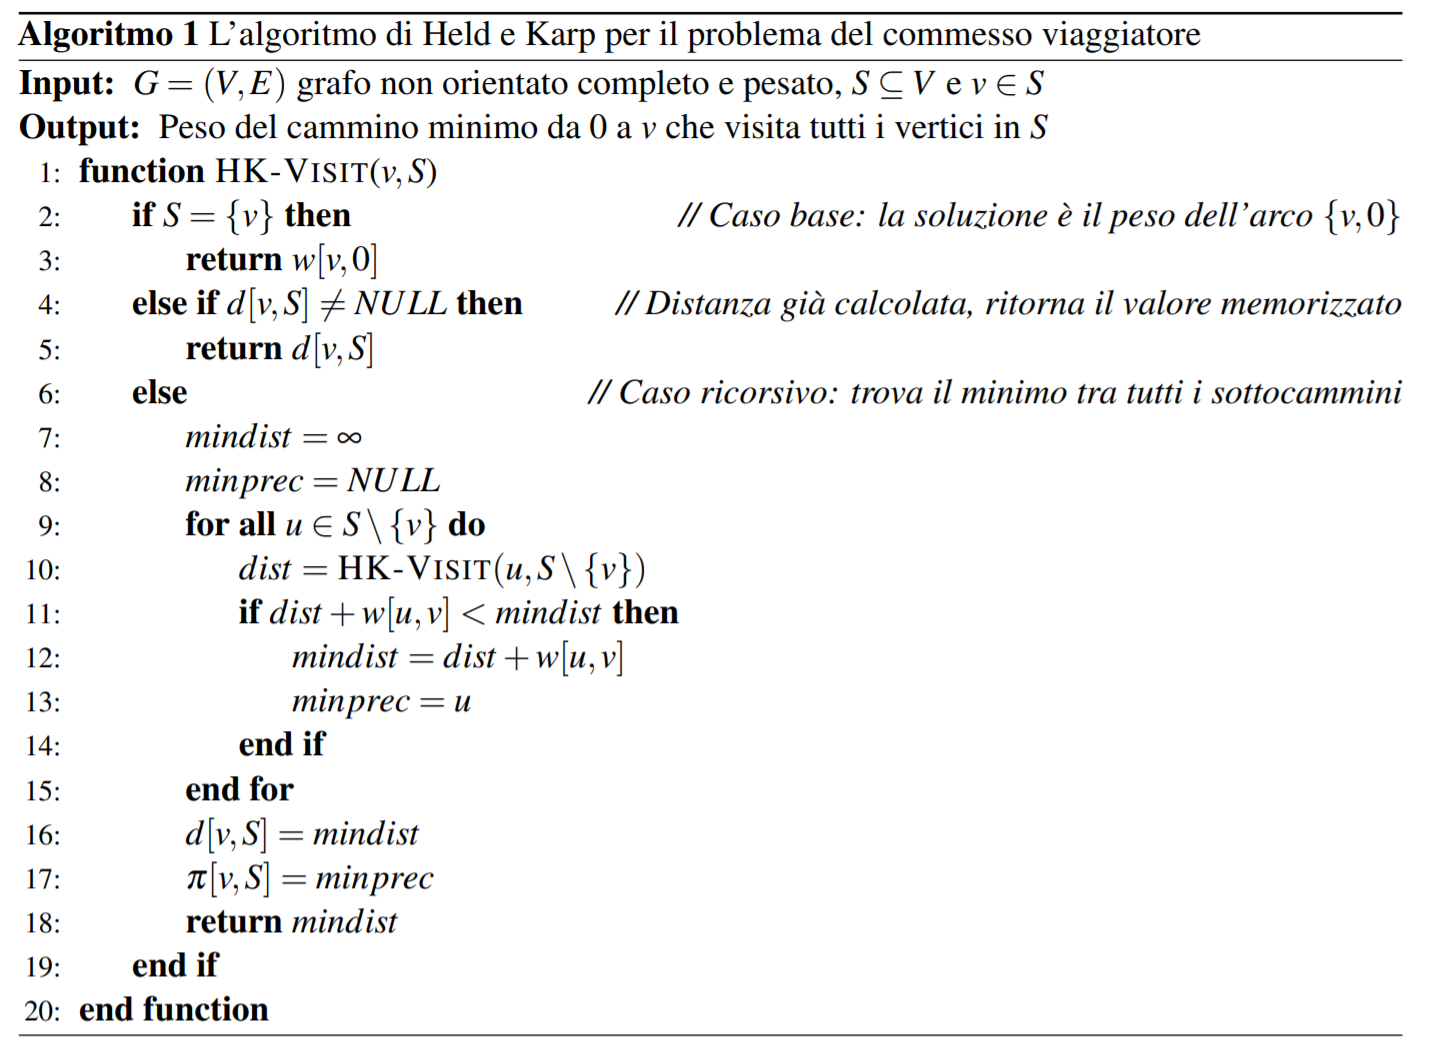
\includegraphics[width=0.9\textwidth]{./images/HeldKarpPseudocode.png}
	\caption{Pseudocodice dell'algoritmo Held-Karp.}
	\label{fig:heldkarp-pseudocode}
\end{figure}

\noindent Il listato \ref{listing:held-karp} contiene la nostra implementazione dell'algoritmo, step per step.

\begin{listing}[!ht]
\begin{minted}{c++}
// HeldKarp.h

int held_karp_tsp_rec_bits_helper(timeout::timeout_signal& signal,
                                  DistanceMatrix<int>& distance_matrix,
                                  held_karp_dp_bits_t& C,
                                  utils::ull bits, size_t v = 0) {
    
    // Caso base: c'è solo un nodo nel subpath
    if (utils::is_singleton(bits, v)) {
        return distance_matrix.at(v, 0);
    }

    // Distanza già calcolata, ritorna il valore memorizzato
    if (C.count({bits, v})) {
        return C[{bits, v}];
    }
    
    // Caso ricorsivo
    int min_dist = std::numeric_limits<int>::max();
    const utils::ull difference = utils::reset_bit(bits, v);
    const size_t n = distance_matrix.size();

    // for all u in S\{v}
    utils::for_each(difference, n, [&](const size_t bit) {
        int dist = held_karp_tsp_rec_bits_helper(signal, distance_matrix, C,
                                                 difference, bit);
        int tmp_dist = dist + distance_matrix.at(v, bit);

        if (tmp_dist < min_dist) {
            min_dist = tmp_dist;
        }

        // Timeout scaduto: ritorna il miglior risultato ottenuto fino ad ora
        return !signal.is_expired();
    });

    C[{bits, v}] = min_dist;
    return min_dist;
}

\end{minted}
\caption{Implementazione di Held e Karp con BitMasking. I commenti del file originale sono stati omessi per una maggiore compattezza.}
\label{listing:held-karp}
\end{listing}

\subsubsection{Osservazioni}

\begin{itemize}
    \item Abbiamo voluto riportare qui la versione con BitMasking a 64 bit, la versione con DynamicBitMasking è simile. Il controllo su quale delle due implementazioni usare è fatto prima di lanciare la funzione di ricorsione appropriata.\\
\end{itemize}

\newpage


\subsection{Farthest Insertion}

La versione vista a lezione di Farthest Insertion prevede i seguenti step:

\begin{enumerate}
    \item ---
    \item ---
\end{enumerate}

\noindent Il listato \ref{listing:farthest-insertion} contiene la nostra implementazione dell'algoritmo, step per step.

\begin{listing}[!ht]
\begin{minted}{c++}

\end{minted}
\caption{Implementazione di Farthest Insertion. I commenti del file originale sono stati omessi per una maggiore compattezza.}
\label{listing:farthest-insertion}
\end{listing}

\subsubsection{Osservazioni}
\begin{itemize}
    \item ----\\

\end{itemize}
